\documentclass[../report.tex]{subfiles}
\begin{document}
\graphicspath{{img/}{../img/}}

The internet is not like old phone lines which needed to be connected directly, instead much information travels through the same lanes. In order to process this information...

Since all but one service operations on ShareIt are private, it is important to discuss how this is handled.

Two consecutive walls will block your way when reaching ShareIt; First a token validation and secondly a user credential validation. \\

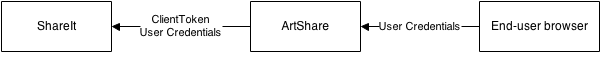
\includegraphics[width=\linewidth]{./AccessControlDeployment.png}

\subsection{Token validation}

The token validation is implemented as a means for ShareIt to only allow recognized clients to invoke any operations. This means that ShareIt's database has a Client table against which ShareIt checks incoming tokens. These tokens are very static and do not depend on any communication session, but are created specifically for an implementor to use.

In order to associate a token with a client the token has to be transfered through an encrypted channel. However security is not in scope here, which has the consequence that anybody could sniff the token.

Below is the token which ShareIt associates with ArtShare. The token could be anything digital as long as its' length implicates a brute force attack.

\begin{center}
\texttt{7dac496c534911c0ef47bce1de772502b0d6a6c60b1dbd73c1d3f285f36a0f61}
\end{center}



\subsection{User credential validation}

Operations on ShareIt that are user specific in any way take a \texttt{UserDto}. In these cases the UserDto is validated with the database on it's Username and Password properties. An example is the operation to validate whether a User is registered with the system.

\begin{center}
\texttt{int ValidateUser(UserDTO user, string clientToken);}
\end{center}

While the clientToken has a single purpose, namely to validate clients, the user credential check is multi-functional in the way it determines many types of access rights with the system.


\subsection{Access rights}

\todo{write}


\end{document}